\section{Πειράματα Εύρεσης Δωματίων}
\label{sec:experiments_map_annotation}

Στο πρώτο μέρος των πειραμάτων χρησιμοποιούνται 80 διαφορετικοί χάρτες με σκοπό την μελέτη της ακρίβειας εύρεσης των διάφορων πορτών του χώρου. Οι 74 συλλέχθηκαν από το \cite{li2019houseexpo}, ενώ για τους υπόλοιπους 6 δημιουργήθηκε το αντίστοιχο περιβάλλον στο Gazebo και μετά από την διαδικασία SLAM προέκυψαν τα αντίστοιχα OGM.

Σε όλους τους χάρτες δοκιμάστηκε η υλοποίηση του προηγουμένου κεφαλαίου \ref{section:map_annotation} και μετρήθηκαν 3 συνολικά στοιχεία:

\begin{itemize}
    \setlength\itemsep{-0.2em}
    \item True Positives: σημεία που είναι πόρτες και εντοπίστηκαν σωστά
    \item False Negatives: σημεία που είναι πόρτες αλλά δεν εντοπίστηκαν
    \item False Positives: σημεία που δεν είναι πόρτες αλλά χαρακτηρίστηκαν ως τέτοιες
\end{itemize}

Στο \autoref{fig:rooms_3_ogm_room_detection_example} παρουσιάζονται από δύο παραδείγματα για κάθε περίπτωση. Έστω ότι στον χάρτη αυτό προέκυψαν 4 τελικοί κόμβοι πόρτας (2 μπλε και 2 κόκκινοι). Οι δύο που σημειώνονται με κόκκινο χρώμα πράγματι βρίσκονται σε πόρτες του δωματίου, δηλαδή είναι True Positives. Οι δύο μπλε κόμβοι δεν αποτελούν σημείο πόρτας αν και έχουν χαρακτηριστεί έτσι, επομένως είναι False Positive. Τέλος, στις περιπτώσεις που σημειώνονται με πράσινους κύκλους η διαδικασία απέτυχε να εντοπίσει τις δύο πόρτες, δηλαδή πρόκειται για περιπτώσεις Fasle Negative αποτελεσμάτων.


\begin{figure}[!htb]
    \centering
    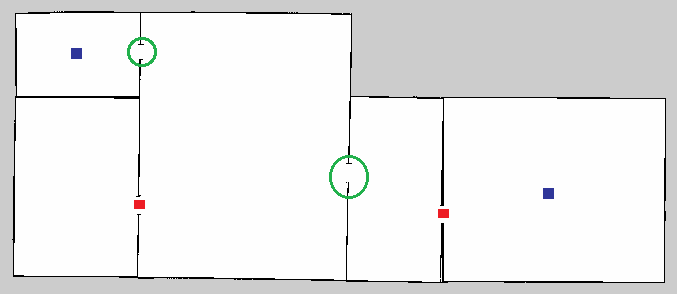
\includegraphics[width=0.8\textwidth]{./images/chapter6/rooms_3_ogm_room_detection_example.png}
    \caption{Παραδείγματα μετρήσεων πειράματος}
    \label{fig:rooms_3_ogm_room_detection_example}
\end{figure}


Τα τελικά αποτελέσματα είναι:
\begin{table}[H]
  \begin{center}
    \caption{Μετρήσεις Εντοπισμού Πορτών}
    \label{tab:room_detection}
    \begin{tabular}{ |>{\columncolor[gray]{0.8}} c | c | }
      \hline
      True Positive & $501$ \\ \hline
      False Negative & $40$ \\ \hline
      False Positive & $149$ \\
      \hline
    \end{tabular}
  \end{center}
\end{table}

Το θετικό συμπέρασμα που προκύπτει είναι ότι η διαδικασία έχει πολύ υψηλό ποσοστό εντοπισμού μιας πόρτας $accuracy = 92.606\%$. Το αρνητικό είναι ότι εμφανίζονται αρκετά συχνά πόρτες σε σημεία που δεν υπάρχουν. Ωστόσο, όπως θα φανεί και από κάποια παραδείγματα δεν είναι τόσο σημαντικό πρόβλημα για δύο λόγους. Πρώτον, πολλές φορές εμφανίζονται παραπάνω πόρτες σε σημέια όπως η μέση ενός διαδρόμου, όπου δεν επηρεάζει αρνητικά την διαδικασία η θεώρηση ενός ακόμη δωματίου. Δεύτερον και σημαντικότερον, η ύπαρξη αυτή προκύπτει εξαιτίας της αναπαράστασης του χώρου. Η συλλογή \cite{li2019houseexpo} περιέχει χάρτες σε μορφή εικόνας png και όχι σε μορφή OGM. Αυτό έχει ως αποτέλεσμα τα σημεία που είναι εκτός των δωματίων, αντί να αντιστοιχούν σε τιμές αγνώστου, αντιστοιχούν σε τιμές εμποδίων. Έτσι, ο αλγόριθμος όταν ελέγχει το ποσοστό κάλυψης της προέκτασης της ευθείας των κοντινότερων εμποδίων δίνει μεγάλες τιμές, κάτι που με κανονική OGM αναπαράσταση δεν θα συνέβαινε. Το επιχείρημα αυτό βασίζεται στο γεγονός ότι και οι έξι OGM χάρτες έχουν 100\% ακρίβεια στον εντοπισμό των πορτών, χωρίς την ύπαρξη λανθασμένων υποδείξεων.

Επομένως, τα δωμάτια ενός χώρου συνδέονται άμεσα με τα χαρακτηριστικά του αντίστοιχου χάρτη. Ο εντοπισμός και διαχωρισμός τους μπορεί να πραγματοποιηθεί με μεγάλη επιτυχία με το αναπτυγμένο σύστημα που εξαρτάται αποκλειστικά από τον εκάστοτε χάρτη.

Στην συνέχεια παρουσιάζονται ορισμένα παραδείγματα χαρτών με τους κόμβους. Οι μπλε κόμβοι αποτελούν τα εκτιμώμενα σημεία πόρτας, τα πράσινα τους υποψήφιους κόμβους πόρτες που απορρίφθηκαν και τα κόκκινα τα υπόλοιπα σημεία του τοπολογικού χάρτη του χώρου.

Στο \ref{fig:room_detection_example_1} επιτεύχθηκε σωστός εντοπισμός των δωματίων. Στο \ref{fig:room_detection_example_2} παρατηρούνται τρεις περιττοί κόμβοι, δύο πάνω αριστερά και ένας κάτω αριστερά. Και οι τρεις προκύπτουν από το γεγονός ότι στο αριστερό μέρος του χώρου υπάρχει ένα τεράστιο εμπόδιο, κάτι που υπό φυσιολογικές συνθήκες θα ήταν άγνωστη περιοχή ή ένα άλλο δωμάτιο. Στο \ref{fig:room_detection_example_3} ο χώρος προσομοιώνει μια πραγματική αποθήκη και η διαδικασία εντοπίζει και τις δύο πόρτες του χώρου. Τέλος, στο \ref{fig:room_detection_example_4} συναντάται ένας πολύ σύνθετος χώρος. Ωστόσο, η διαδικασία εντοπίζει με επιτυχία και τις έξι πόρτες. 

Παρατηρώντας τα παραδείγματα αυτά φαίνεται ότι πράγματι η διαδικασία λειτουργεί με ικανοποιητικά αποτελέσματα σε πολλούς και σύνθετους χώρους όπως είναι μια αποθήκη.


\begin{figure}[!htb]
    \centering
    \begin{subfigure}{0.5\textwidth}
        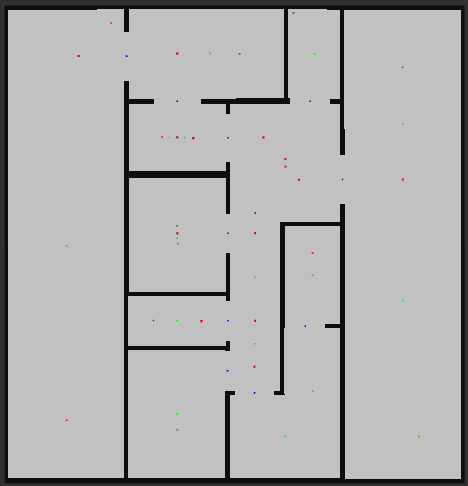
\includegraphics[width=0.9\textwidth]{./images/chapter6/b1c86b70b59c42219161174de6500049.png}
        \caption{Παράδειγμα 1}
        \label{fig:room_detection_example_1}
    \end{subfigure}%
% \end{figure}
% \begin{figure}[!htb]
    \begin{subfigure}{0.5\textwidth}
        \centering
        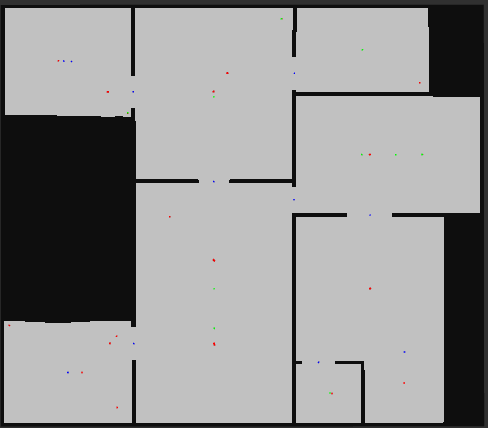
\includegraphics[width=0.9\textwidth]{./images/chapter6/fea87120e90bbffd5e8c42e3b6002165.png}
        \caption{Παράδειγμα 2}
        \label{fig:room_detection_example_2}
    \end{subfigure}
    \begin{subfigure}{0.5\textwidth}
        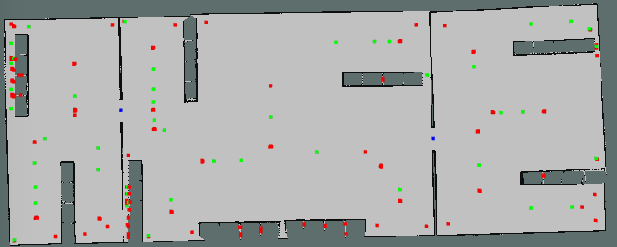
\includegraphics[width=0.9\textwidth]{./images/chapter6/warehouse_2.png}
        \caption{Παράδειγμα 3}
        \label{fig:room_detection_example_3}
    \end{subfigure}%
    \begin{subfigure}{0.5\textwidth}
        \centering
        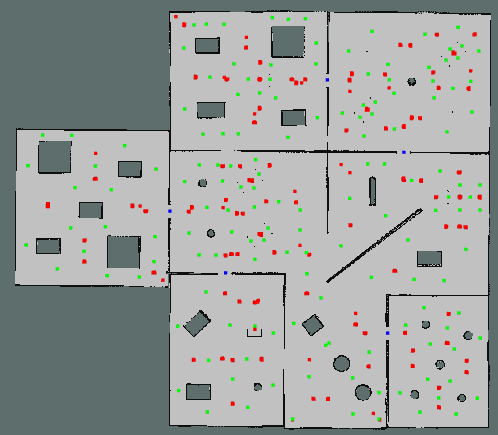
\includegraphics[width=0.9\textwidth]{./images/chapter6/indoor_with_distance_features.png}
        \caption{Παράδειγμα 4}
        \label{fig:room_detection_example_4}
    \end{subfigure}
\end{figure}






